%inicio Ester
\chapter{Skiplists}

\chaplabel{skiplists}

Neste capítulo discutiremos uma bela estrutura de dados: a skiplist,
que possui diversas de aplicações.  Usando uma skiplist, podemos implementar uma
#Lista# que tenha tempo de $O(\log n)$ para implementações de #get(i)#, #set(i,x)#,
#add(i,x)#, e #remove(i)#. Nós também podemos implementar uma #SSet# em que
todas as operação são executadas com tempo esperado de $O(\log #n#)$.
%Finally, a skiplist can be used to implement a #Rope# in which all
%operations run in $O(\log #n#)$ time.

A eficiência das skiplists se baseia no uso da randomização.
Quando um novo elemento é adicionado à skilist, ela utiliza lançamentos aleatórios
de moeda para determinar a altura do novo elemento.  O desempenho das
skiplists é expresso em termos do tempo de execução esperado e do tamanho do
caminho. Esta expectativa é baseada nos lançamentos aleatórios de moeda usados
pela skiplist.  Na implementação, os lançamentos aleatórios de moedas usados pela
skiplist são simulados usando um gerador de números  (ou bits) pseudo aleatórios.

\section{A Estrutura Básica}

\index{skiplist}%
Conceitualmente, uma skiplist é uma sequência de listas simplesmente encadeadas
$L_0,\ldots,L_h$. Cada lista $L_r$ contém um subconjunto de itens 
em $L_{r-1}$.  Começamos com a lista inicial $L_0$ que contém #n#
itens e construímos $L_1$ a partir de $L_0$, $L_2$ a partir de $L_1$, e assim por diante.

Os itens em $L_r$ são obtidos lançando a moeda para cada elemento, #x#,
em $L_{r-1}$ e incluindo #x# em $L_r$ se a moeda der cara.
Este processo termina quando criamos uma lista $L_r$ que está vazia.  Um exemplo
de uma skiplist é mostrado na \figref{skiplist}.

\begin{figure}
  \begin{center}
    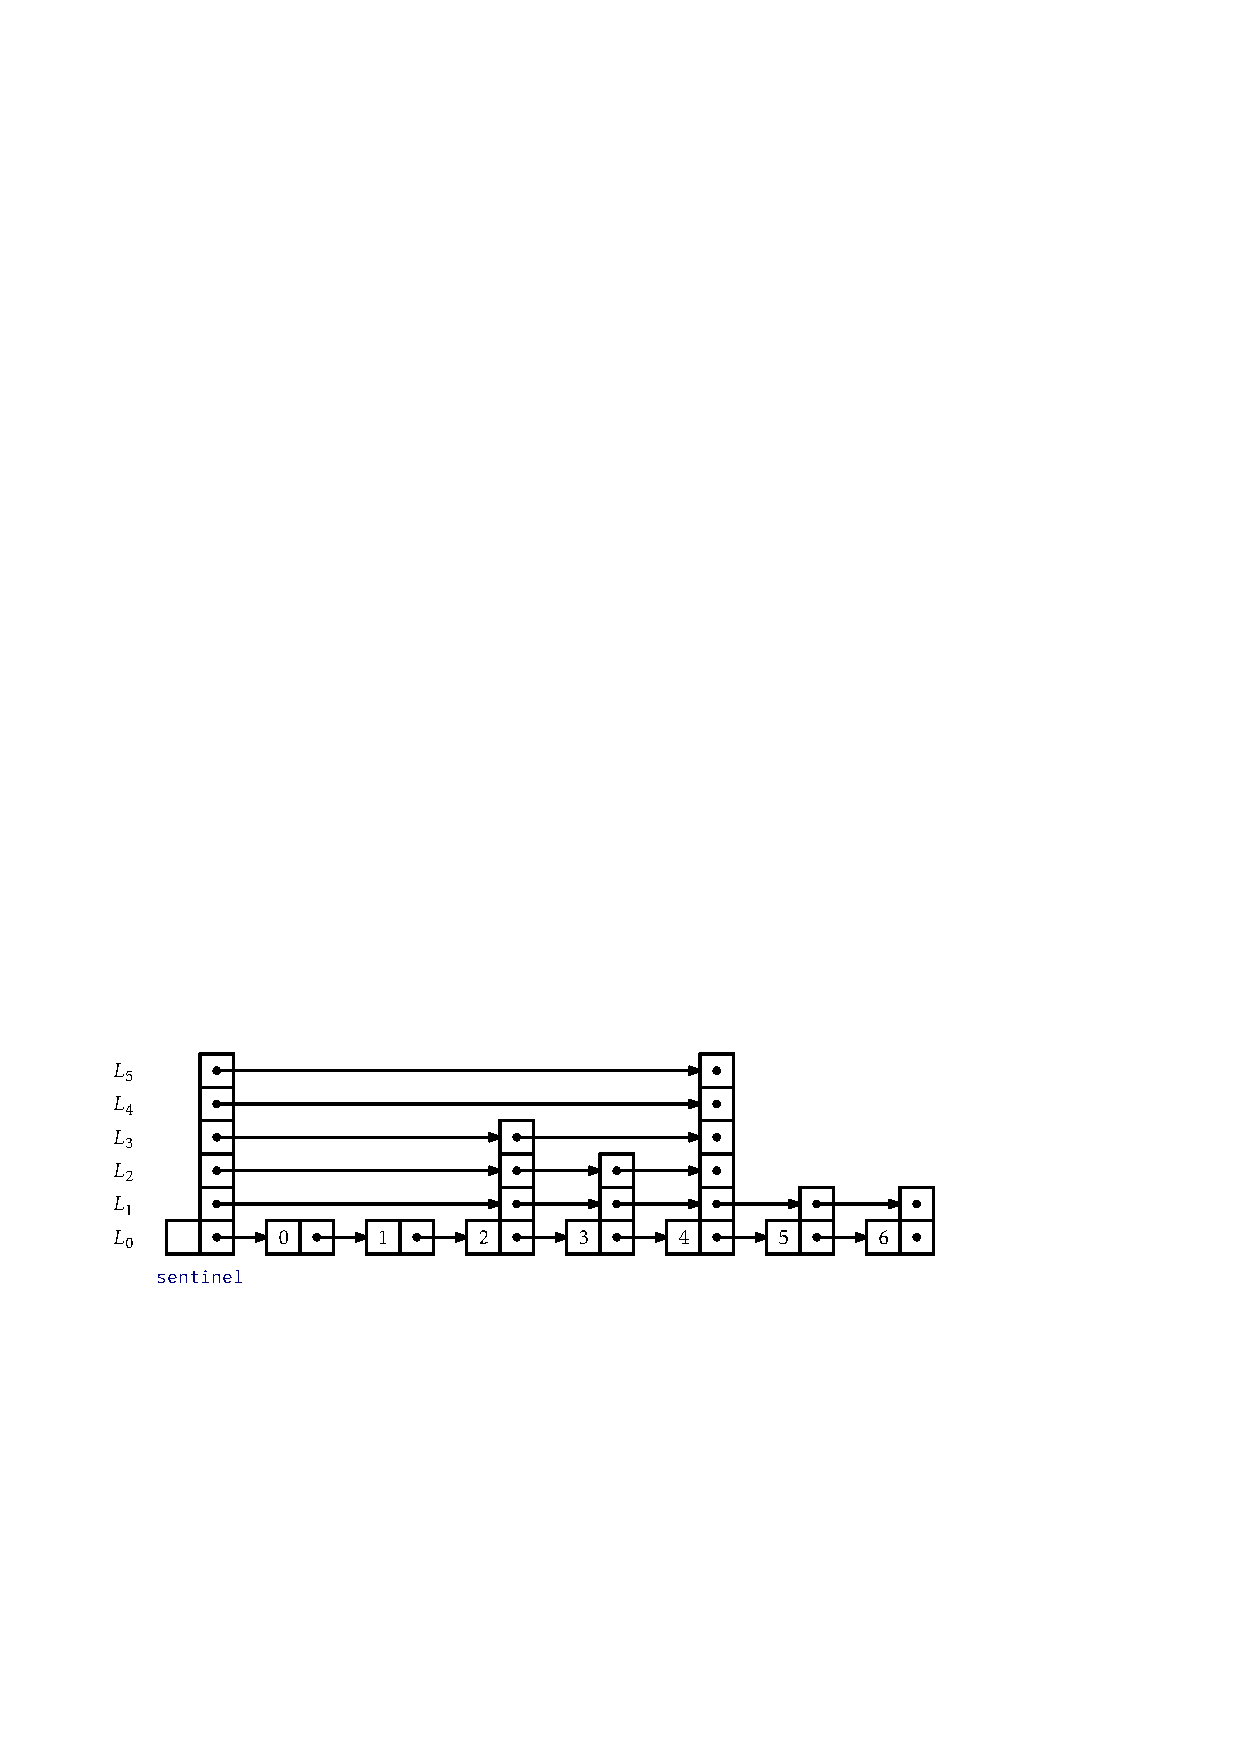
\includegraphics[width=\ScaleIfNeeded]{figs/skiplist}
  \end{center}
  \caption{Uma skiplist com sete elementos.}
  \figlabel{skiplist}
\end{figure}

Para um elemento, #x#, na skiplist, nós chamamos de \emph{height}
\index{height!of a skiplist}%
de #x# o
o valor mais alto de $r$ de modo que #x# apareça em $L_r$.  Assim, por exemplo,
elementos que só aparecem em $L_0$ tem altura $0$.  Se pararmos um momento pra
pensar sobre isso, percebemos que a altura de #x# corresponde
à seguinte experiência:  lance uma moeda repetidamente até aparecer
como coroa. Quantas vezes apareceu cara? A resposta, sem
surpresa, é que a altura esperada de um nó é 1. (Esperamos
lançar a moeda duas vezes antes de aparecer coroa, mas não contamos a última
jogada.) O \emph{height} de uma skiplist é a altura do seu nó mais alto.

No começo de cada lista está um nó especial, chamado de \emph{sentinela},
\index{sentinel node}%
que atua como um pseudo nó (\textit{dummy}) para a lista. A propriedade chave das skiplists
é que existe um caminho curto para busca, chamado de \emph{caminho de busca}, 
\index{caminho de busca!em uma skiplist}%
do
sentinela em $L_h$ para cada nó em $L_0$.  Lembrando como construir
um caminho de busca para o nó, #u#, é fácil (veja \figref{skiplist-searchpath})
:  Comece no canto superior esquerdo da skiplist (o sentinela em $L_h$)
e sempre vá para a direita, a menos que ultrapasse #u#, nesse caso você
deve dar uma passo para a lista de baixo.

Mais precisamente, para construir um caminho de busca para o nó #u# em $L_0$,
começaremos pelo sentinela, #w#, em $L_h$.  Em seguida, verificamos #w.next#.
Se #w.next# contém um elemento que aparece antes de #u# em $L_0$, então
nós ajustamos $#w#=#w.next#$.  Caso contrário, movemos para baixo e continuamos a busca
da ocorrência de#w# na lista $L_{h-1}$.  Continuamos assim
até chegar ao antecessor de #u# em $L_0$. 
\begin{figure}
  \begin{center}
    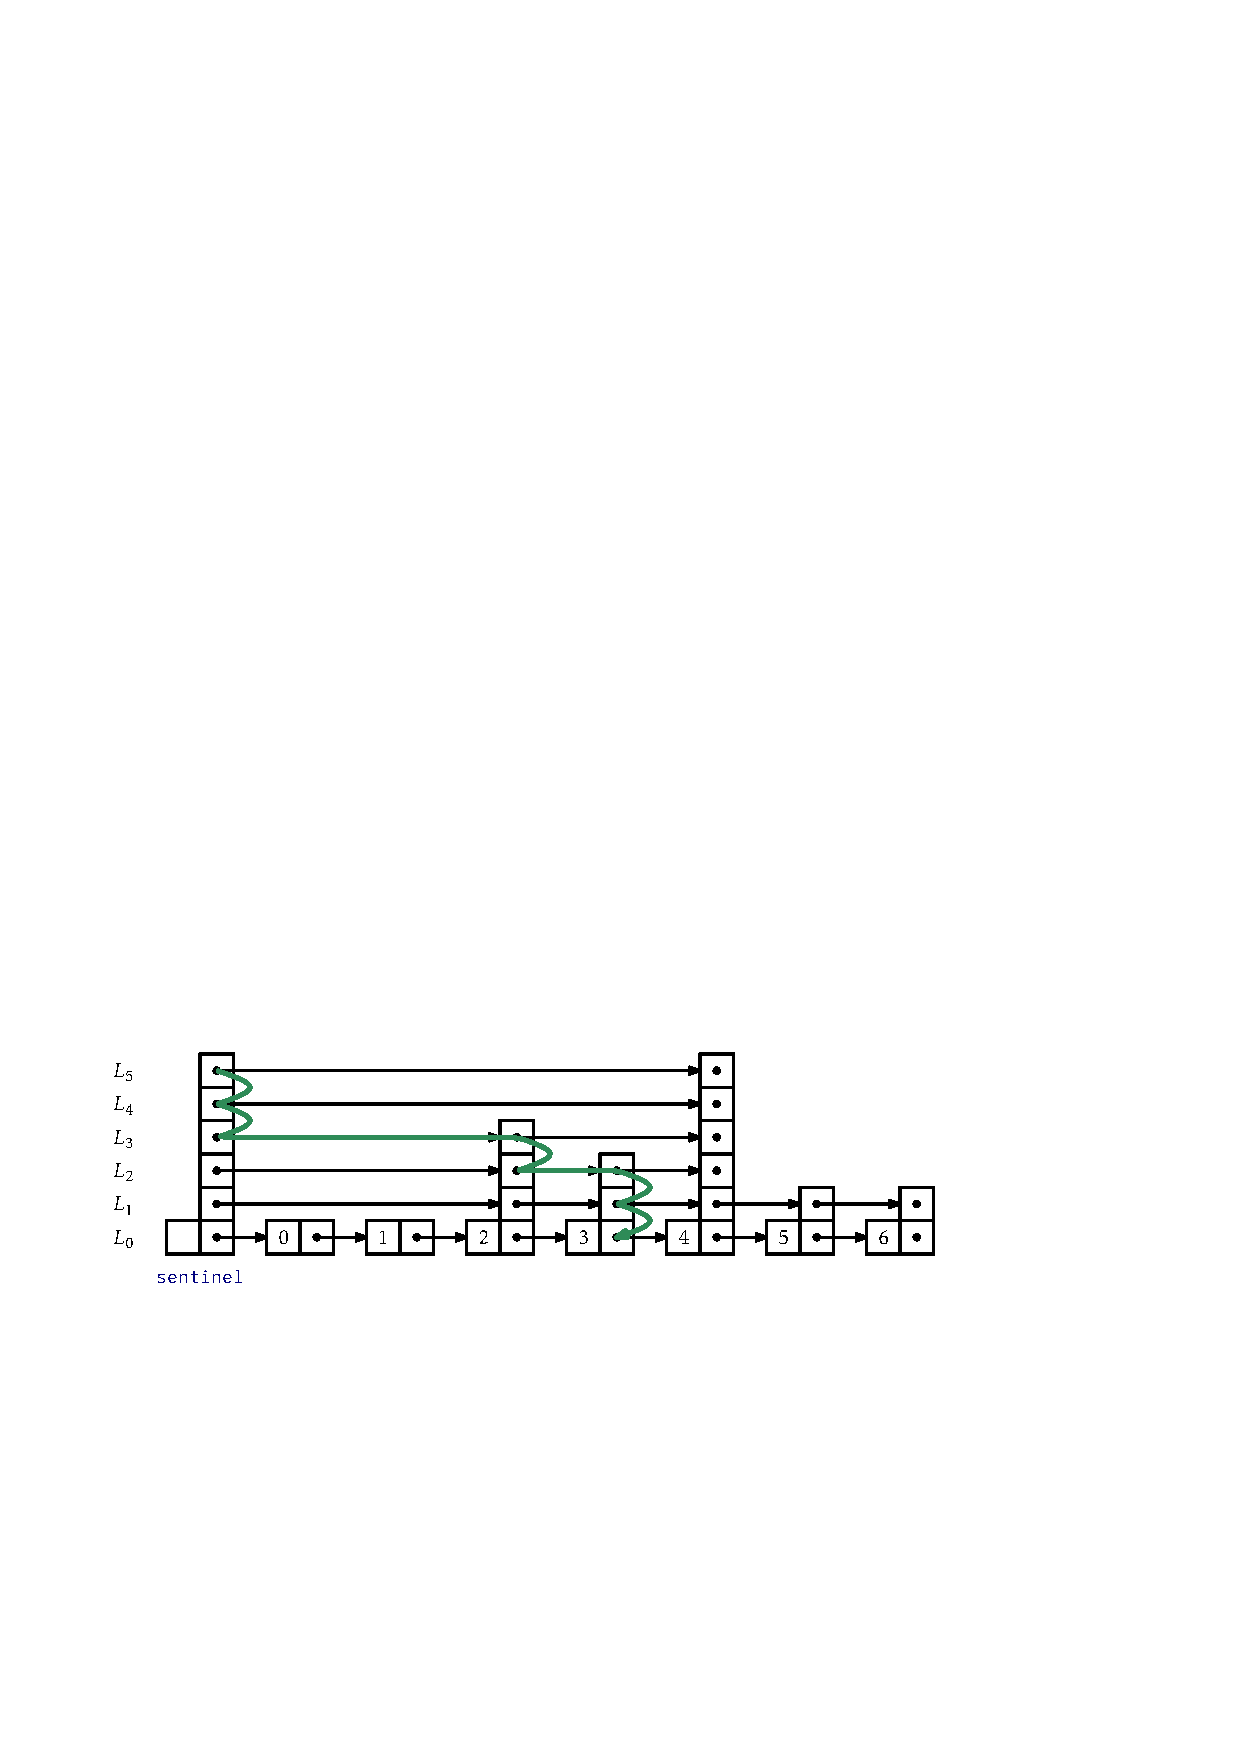
\includegraphics[width=\ScaleIfNeeded]{figs/skiplist-searchpath}
  \end{center}
  \caption{Caminho de busca para o nó que contém o valor $4$ em uma skiplist.}
  \figlabel{skiplist-searchpath}
\end{figure}

O resultado a seguir, que vamos provar em \secref{skiplist-analysis},
mostra que o caminho de busca é bastante curto:

\begin{lem}\lemlabel{skiplist-searchpath}
	O comprimento esperado do caminho de busca para qualquer nó, #u#, em $L_0$ é de no máximo $2\log #n# + O(1) = O(\log #n#)$.
\end{lem}

Uma maneira eficiente em termos de espaço para implementar uma skiplist é definir um #Node#, #u#, consistindo em um valor de dados, #x# e um array, #next#, de ponteiros, onde #u.next[i]# aponta para o sucessor de #u# na lista $L_{#i#}$. Desta forma, os dados, #x#, em um nó são \javaonly{referenciados}\cpponly{armazenados}\pcodeonly{referenciados} apenas uma vez, embora #x# possa aparecer em várias listas.

\javaimport{ods/SkiplistSSet.Node<T>}
\cppimport{ods/SkiplistSSet.Node}

As próximas duas seções deste capítulo abordam duas aplicações diferentes
de skiplists. Em cada uma dessas aplicações, $L_0$ armazena a estrutura principal  (uma lista de elementos ou um conjunto de elementos ordenados).
A principal diferença entre essas estruturas é a forma como
um caminho de busca é navegado; em particular, elas se diferem em como é decidido  se um caminho de busca deve descer em $L_{r-1}$ ou ir para a direita dentro de  $L_r$.

\section{#SkiplistSSet#: Uma #SSet# eficiente}
\seclabel{skiplistset}

\index{SkiplistSSet@#SkiplistSSet#}%
Uma #SkiplistSSet# usa uma skiplist para implementar a interface #SSet#. Quando usada desta maneira, a lista $L_0$ armazena os elementos de #SSet# de forma ordenada. O método #find(x)# funciona seguindo o caminho de busca para o menor valor #y# tal que $#y#\ge#x#$:

\codeimport{ods/SkiplistSSet.find(x).findPredNode(x)}

Seguir o caminho de busca para #y# é fácil. Quando situado em algum nó, #u#, em $L _{#r#}$, olhamos diretamente para #u.next[r].x#, se $#x#>#u.next[r].x#$, então damos um passo à direita em $L_{#r#}$. Caso contrário, descemos para $L_{#r#-1}$. Cada passo (para direita ou descendo) nesta pesquisa leva um tempo constante; assim, para \lemref{skiplist-searchpath}, o tempo de execução esperado de #find(x)# é de $O(\log#n#)$.

Antes de poder adicionar um elemento a #SkipListSSet#, precisamos de um método para simular o lançamento de moedas que determina a altura, #k#, de um novo nó.
Fazemos isso escolhendo um número inteiro aleatório, #z#, e contando o número de $1$s na representação binária de #z#: \footnote {Este método não reproduz exatamente a experiência de lançar moedas, uma vez que o valor de #k# será sempre inferior ao número de bits em um #int#. Contudo, isso terá um impacto insignificante, a menos que o número de elementos na estrutura seja muito maior do que $2^{32}=4294967296$.}

\codeimport{ods/SkiplistSSet.pickHeight()}

Para implementar o método #add(x)# na #SkiplistSSet# procuramos #x# e então colocamos #x# em algumas listas $L_0$, \ldots,$L_{#k#}$, onde #k# é selecionado usando o método #pickHeight()#. A maneira mais fácil de fazer isso é usar um array, #stack#, que acompanha os nós em que o caminho de busca desce de alguma lista $L_{#r#}$ para $L_{#r#-1}$.
Mais precisamente, #stack[r]# é o nó em $L_{#r#}$ onde o caminho de busca
prosseguiu para $L_{#r#-1}$. Os nós que modificamos para inserir #x# são precisamente os nós $#stack[0]#,\ldots,#stack[k]# $. O código seguinte implementa este algoritmo para #add(x)#:
\label{pg:skiplist-add}
\codeimport{ods/SkiplistSSet.add(x)}

\begin{figure}
  \begin{center}
    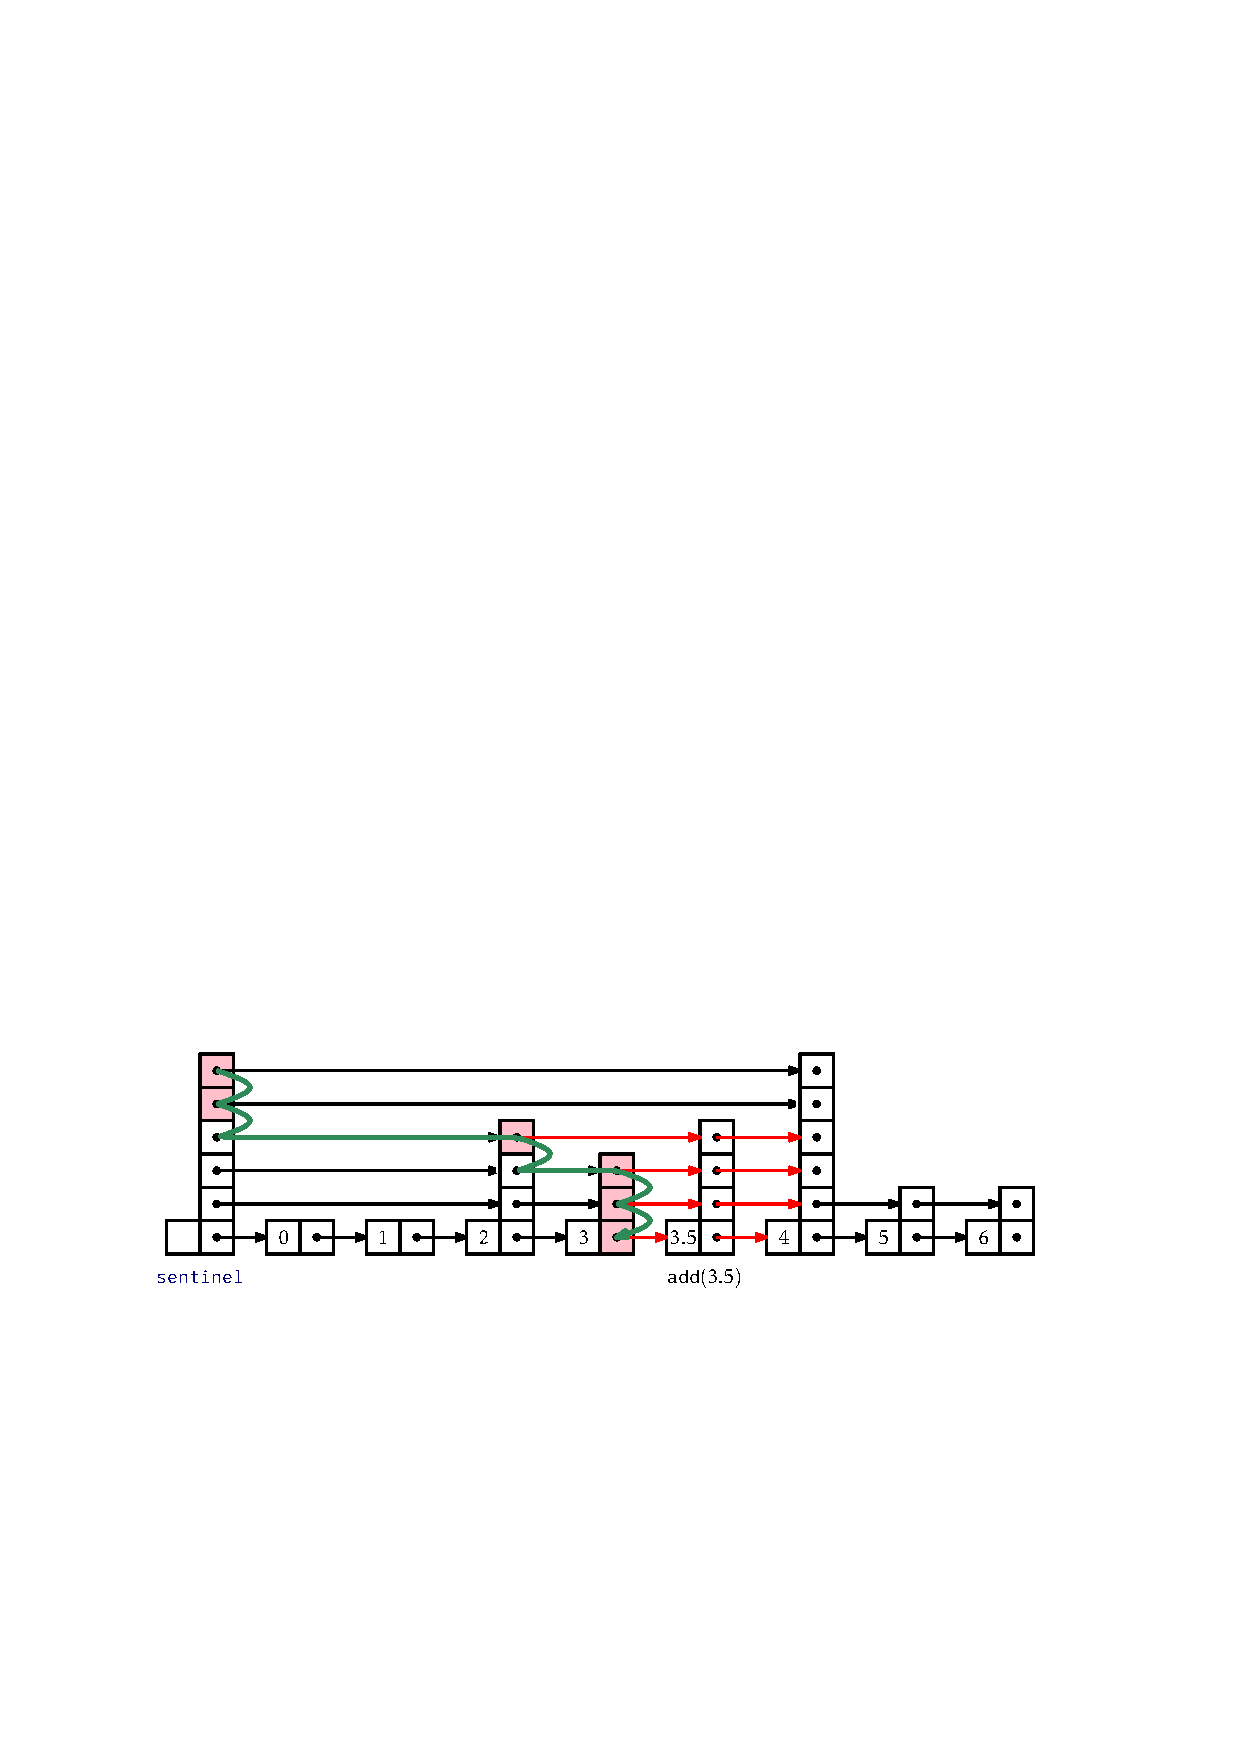
\includegraphics[width=\ScaleIfNeeded]{figs/skiplist-add}
  \end{center}
  \caption[Adding to a skiplist]{Adicionando o nó contendo o valor $3.5$ a uma skiplist.  Os nós armazenados em #stack#
  estão marcados.}
  \figlabel{skiplist-add}
\end{figure}

A remoção de um elemento, #x#, é feita de forma semelhante, exceto que não há
necessidade do #stack# para manter o controle do caminho de busca.  A remoção
pode ser feita enquanto seguimos o caminho de busca.  Procuramos por #x#
e cada vez que a pesquisa se move para baixo a partir do nó #u#, verificamos se
$#u.next.x#=#x#$ e, em caso afirmativo, desligamos #u# da lista:
\codeimport{ods/SkiplistSSet.remove(x)}

\begin{figure}
	\begin{center}
		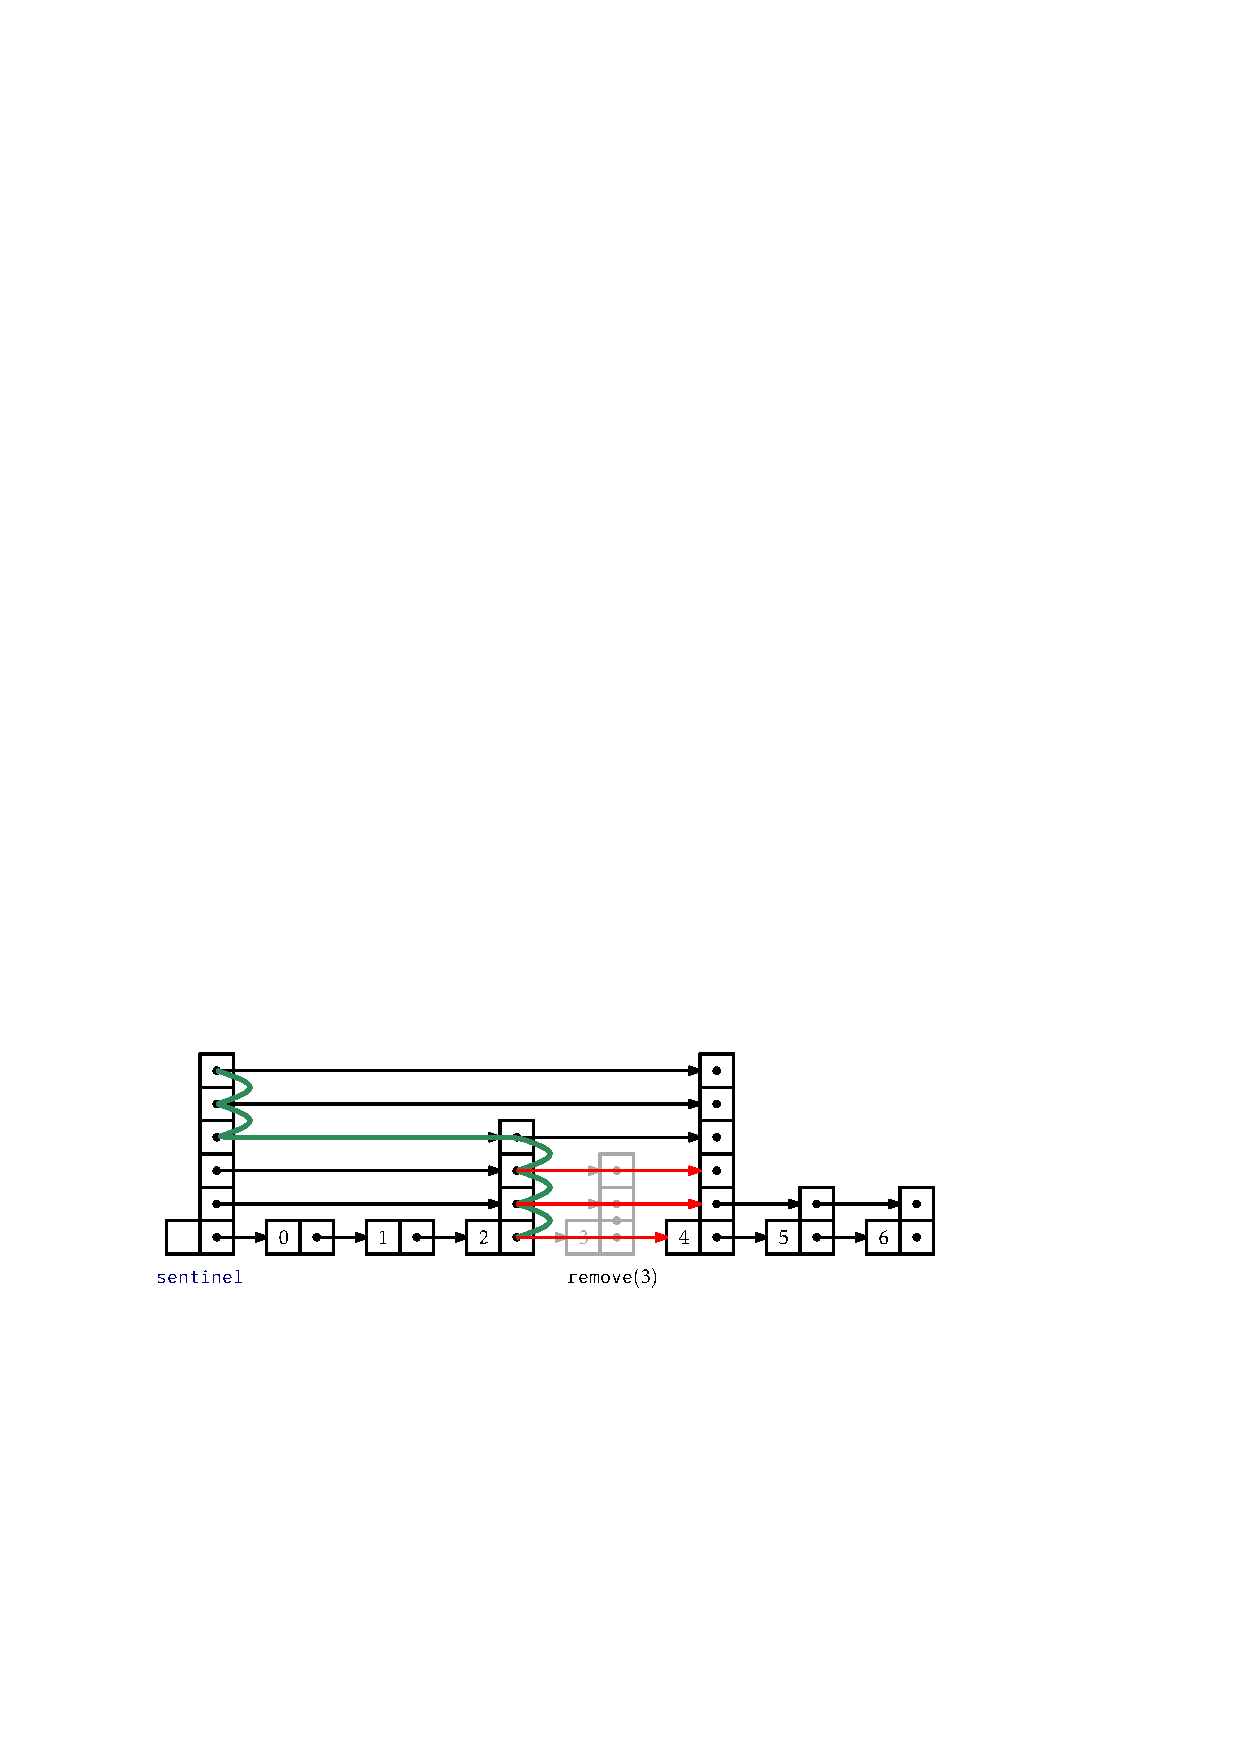
\includegraphics[width=\ScaleIfNeeded]{figs/skiplist-remove}
	\end{center}
	\caption{Removendo o nó que contém o valor $3$ da skiplist.}
	\figlabel{skiplist-remove}
\end{figure}

\subsection{Resumo}

O seguinte teorema resume o desempenho de uma skiplists quando usada para
implementar conjuntos ordenados:

\begin{thm}\thmlabel{skiplist}
	#SkiplistSSet# implementa a interface #SSet#. Uma #SkiplistSSet# suporta
	as operações #add(x)#, #remove(x)#, e #find(x)# em um tempo esperado
	$O(\log #n#)$ por operação.
\end{thm}

\section{#SkiplistList#: Uma #Lista# de acesso aleatório eficiente}
\seclabel{skiplistlist}

\index{SkiplistList@#SkiplistList#}%
Uma #SkiplistList# implementa a interface #List# usando uma estrutura
skiplist.  Em uma #SkiplistList#, $L_0$ contém os elementos da
lista na ordem em que aparecem na lista.   Como em uma #SkiplistSSet#,
os elementos podem ser adicionados, removidos, e acessados em um tempo
$O(\log #n#)$.

Para que isso seja possível, precisamos de uma maneira para seguir o caminho de busca para
o #i#ésimo elemento em $L_0$. A maneira mais fácil de fazer isso é definir
o conceito de \emph{comprimento} de uma aresta em uma lista, $L_{#r#}$.
Definimos o tamanho de cada aresta em $L_{0}$ como 1.  o tamanho de uma aresta, #e#,
em $L_{#r#}$, $#r#>0$, é definido como a soma dos tamanhos das arestas abaixo de #e#
em $L_{#r#-1}$.  De forma equivalente, o tamanho de #e# é
o número de arestas de $L_0$ abaixo de #e#.  Veja \figref{skiplist-lengths} para
um exemplo de uma skiplist mostrando o tamanho de suas arestas.  Uma vez que
as arestas das skiplists são armazenados em arrays, os tamanhos podem ser armazenados da mesma maneira:

\begin{figure}
	\begin{center}
		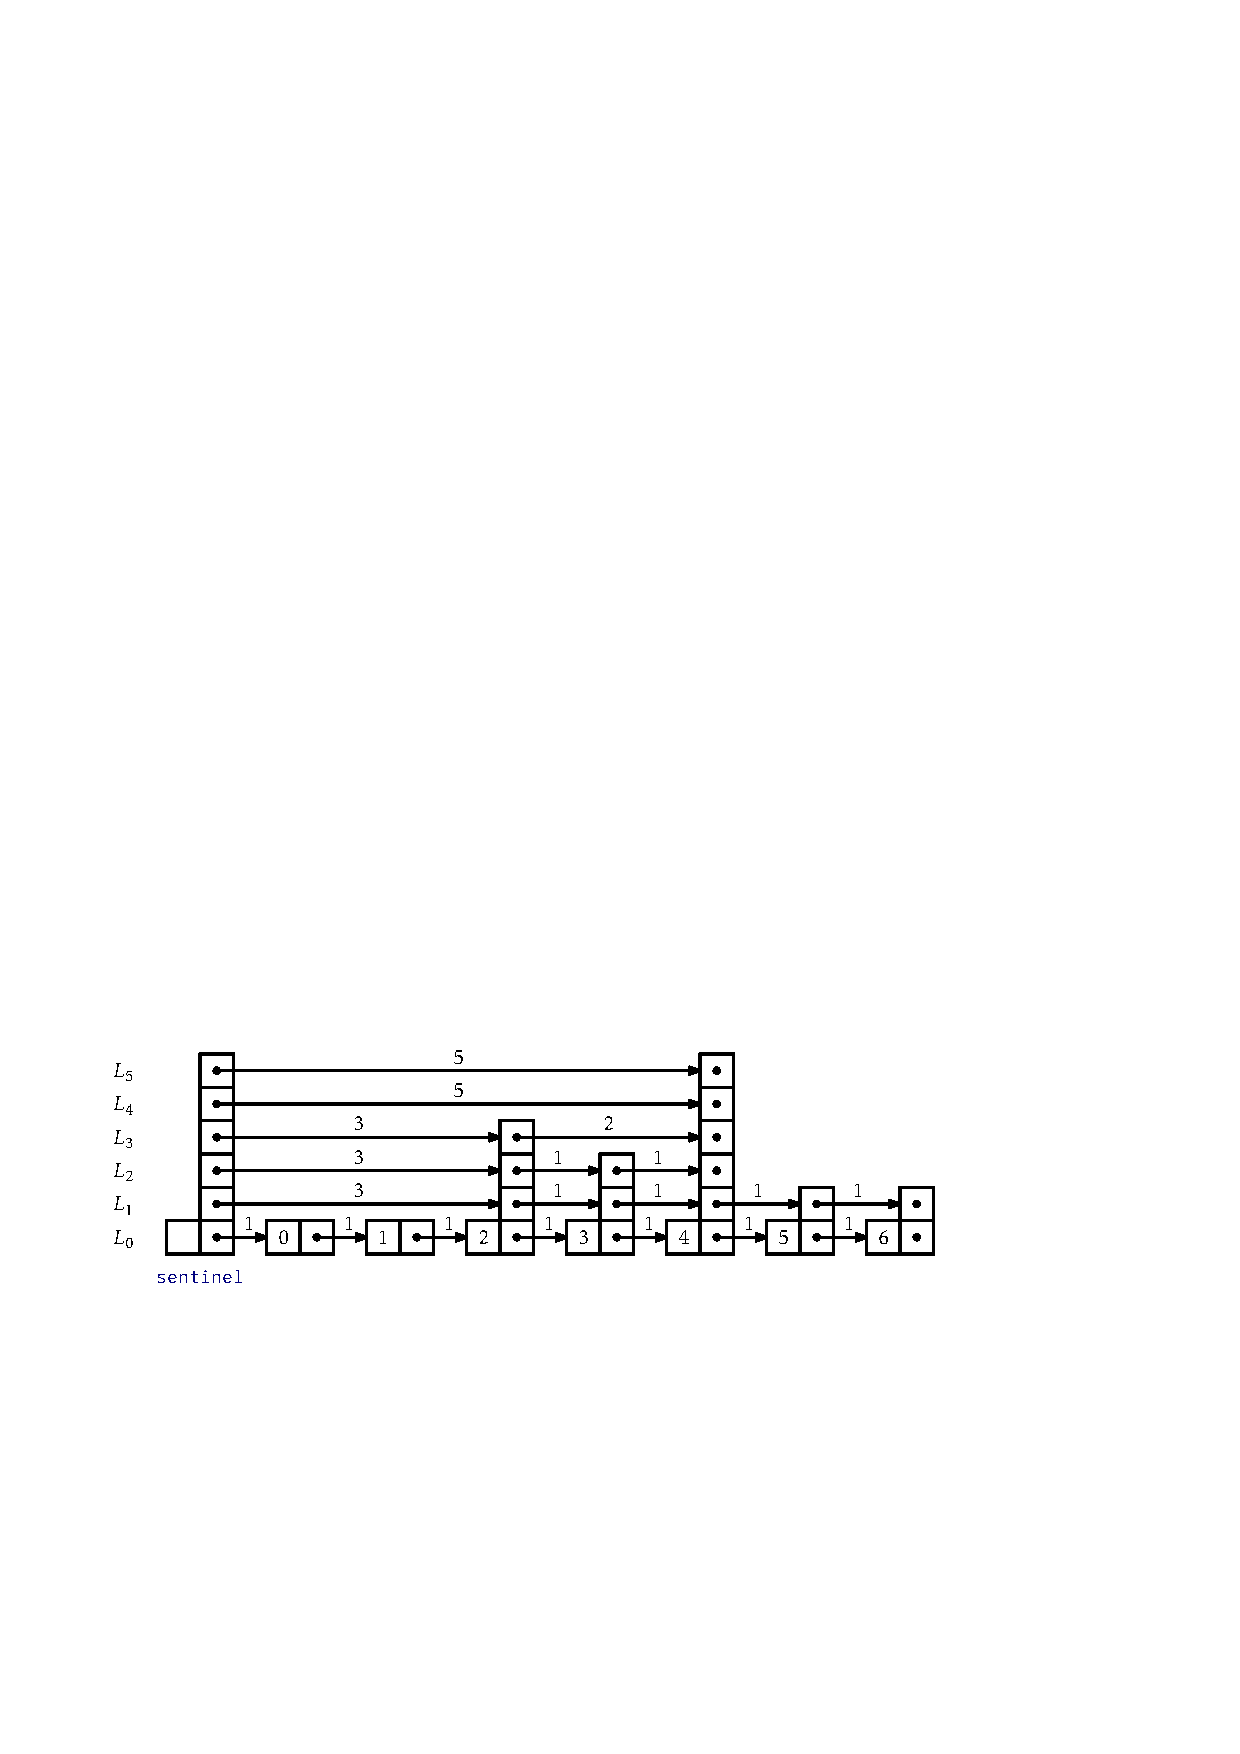
\includegraphics[width=\ScaleIfNeeded]{figs/skiplist-lengths}
	\end{center}
	\caption{Os tamanhos das arestas em uma skiplist.}
	\figlabel{skiplist-lengths}
\end{figure}

\javaimport{ods/SkiplistList.Node}
\cppimport{ods/SkiplistList.Node}

A propriedade útil desta definição de tamanho é que, se estamos
em um nó na posição #j# em $L_0$ e seguimos uma
aresta de tamanho $\ell$, então movemos para um nó cuja posição, em $L_0$,
é $#j#+\ell$.  Desta forma, enquanto seguimos um caminho de busca, podemos manter
o controle da posição, #j#, do nó atual em $L_0$.  Em um
nó, #u#, em $L_{#r#}$, vamos para a direita se #j# mais o tamanho de
#u.next[r]# é menor que #i#. Caso contrário, desceremos para $L_{#r#-1}$.

\codeimport{ods/SkiplistList.findPred(i)}
\codeimport{ods/SkiplistList.get(i).set(i,x)}

Como a parte mais difícil das operações #get(i)# e #set(i,x)# é
encontrar o #i#-ésimo nó em $L_0$, essas operações são executadas em
um tempo $O(\log #n#)$.

Adicionar um elemento a uma #SkiplistList# em uma posição, #i#, é relativamente
simples.  Ao contrário do que acontece em uma #SkiplistSSet#, temos certeza que um novo
nó será realmente adicionado, para que possamos realizar a adição ao mesmo tempo
em que buscamos a localização do novo nó. Primeiramente, pegamos a altura, #k#,
do nó recentemente inserido, #w#, e então avançamos o caminho de busca para #i#.
Toda vez que o caminho de busca desce de $L_{#r#}$ com $#r#\le #k#$,
juntamos #w# em $L_{#r#}$.  O único cuidado extra necessário é assegurar que
o comprimento das arestas seja atualizado devidamente.  Veja \figref{skiplist-addix}.

\begin{figure}
	\begin{center}
		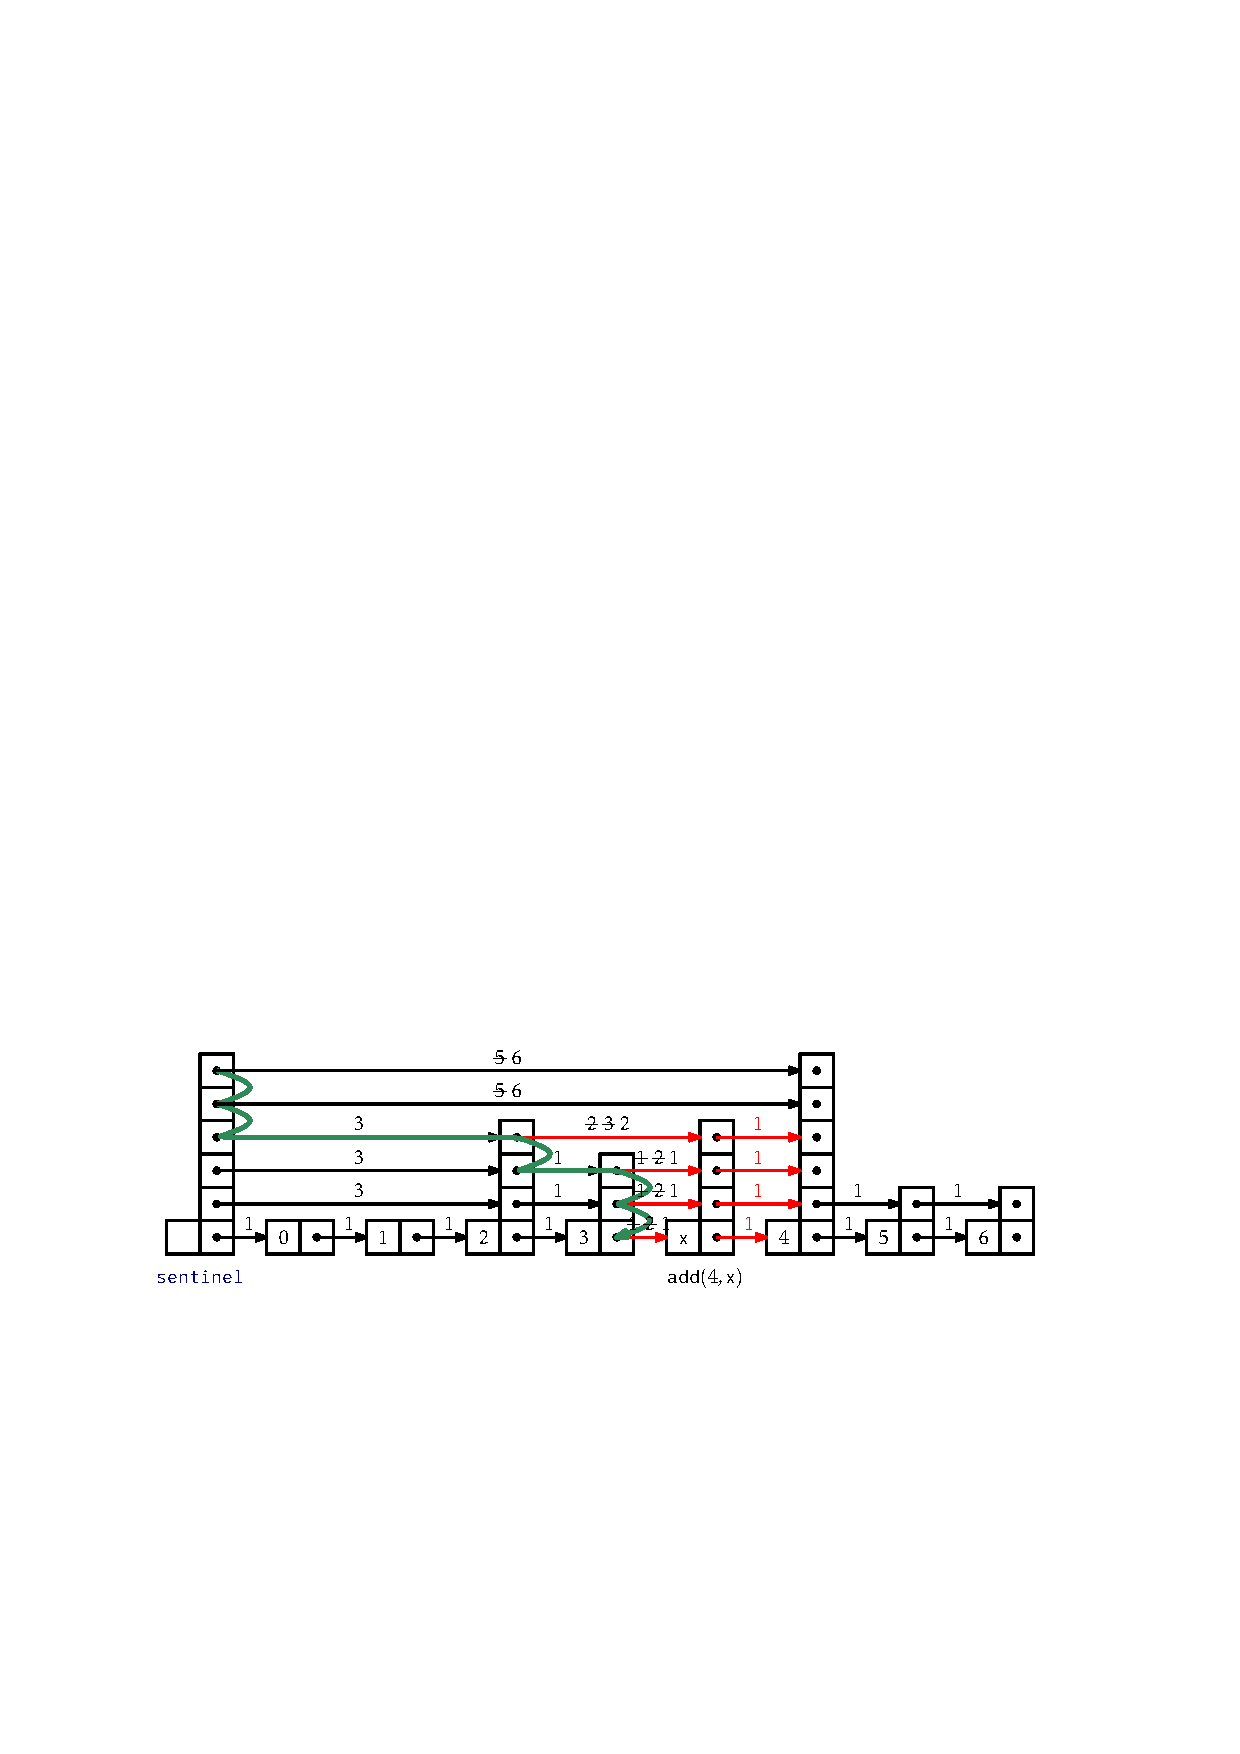
\includegraphics[width=\ScaleIfNeeded]{figs/skiplist-addix}
	\end{center}
	\caption[Adding to a SkiplistList]{Adicionando um elemento em uma #SkiplistList#.}
	\figlabel{skiplist-addix}
\end{figure}

Note que, cada vez que o caminho de busca desce um nó, #u#, em $L_{#r#}$,
o comprimento da aresta #u.next[r]# aumenta em um, uma vez que estamos adicionando
um elemento abaixo desta aresta na posição #i#.  Unir o nó #w# entre dois nós,
#u# e #z#, funciona como mostrado na \figref{skiplist-lengths-splice}. Enquanto
seguimos o caminho de busca, já estamos cientes da posiçao,
#j#, de #u# em $L_0$.  Portanto,sabemos que o comprimento da aresta de
#u# a #w# é $#i#-#j#$.  Também podemos deduzir o comprimento da aresta
de #w#  a #z# através do comprimento, $\ell$, da aresta de #u# a #z#.
Assim sendo, podemos juntar em #w# e atualizar os comprimentos das arestas em
tempo constante.

\begin{figure}
	\begin{center}
		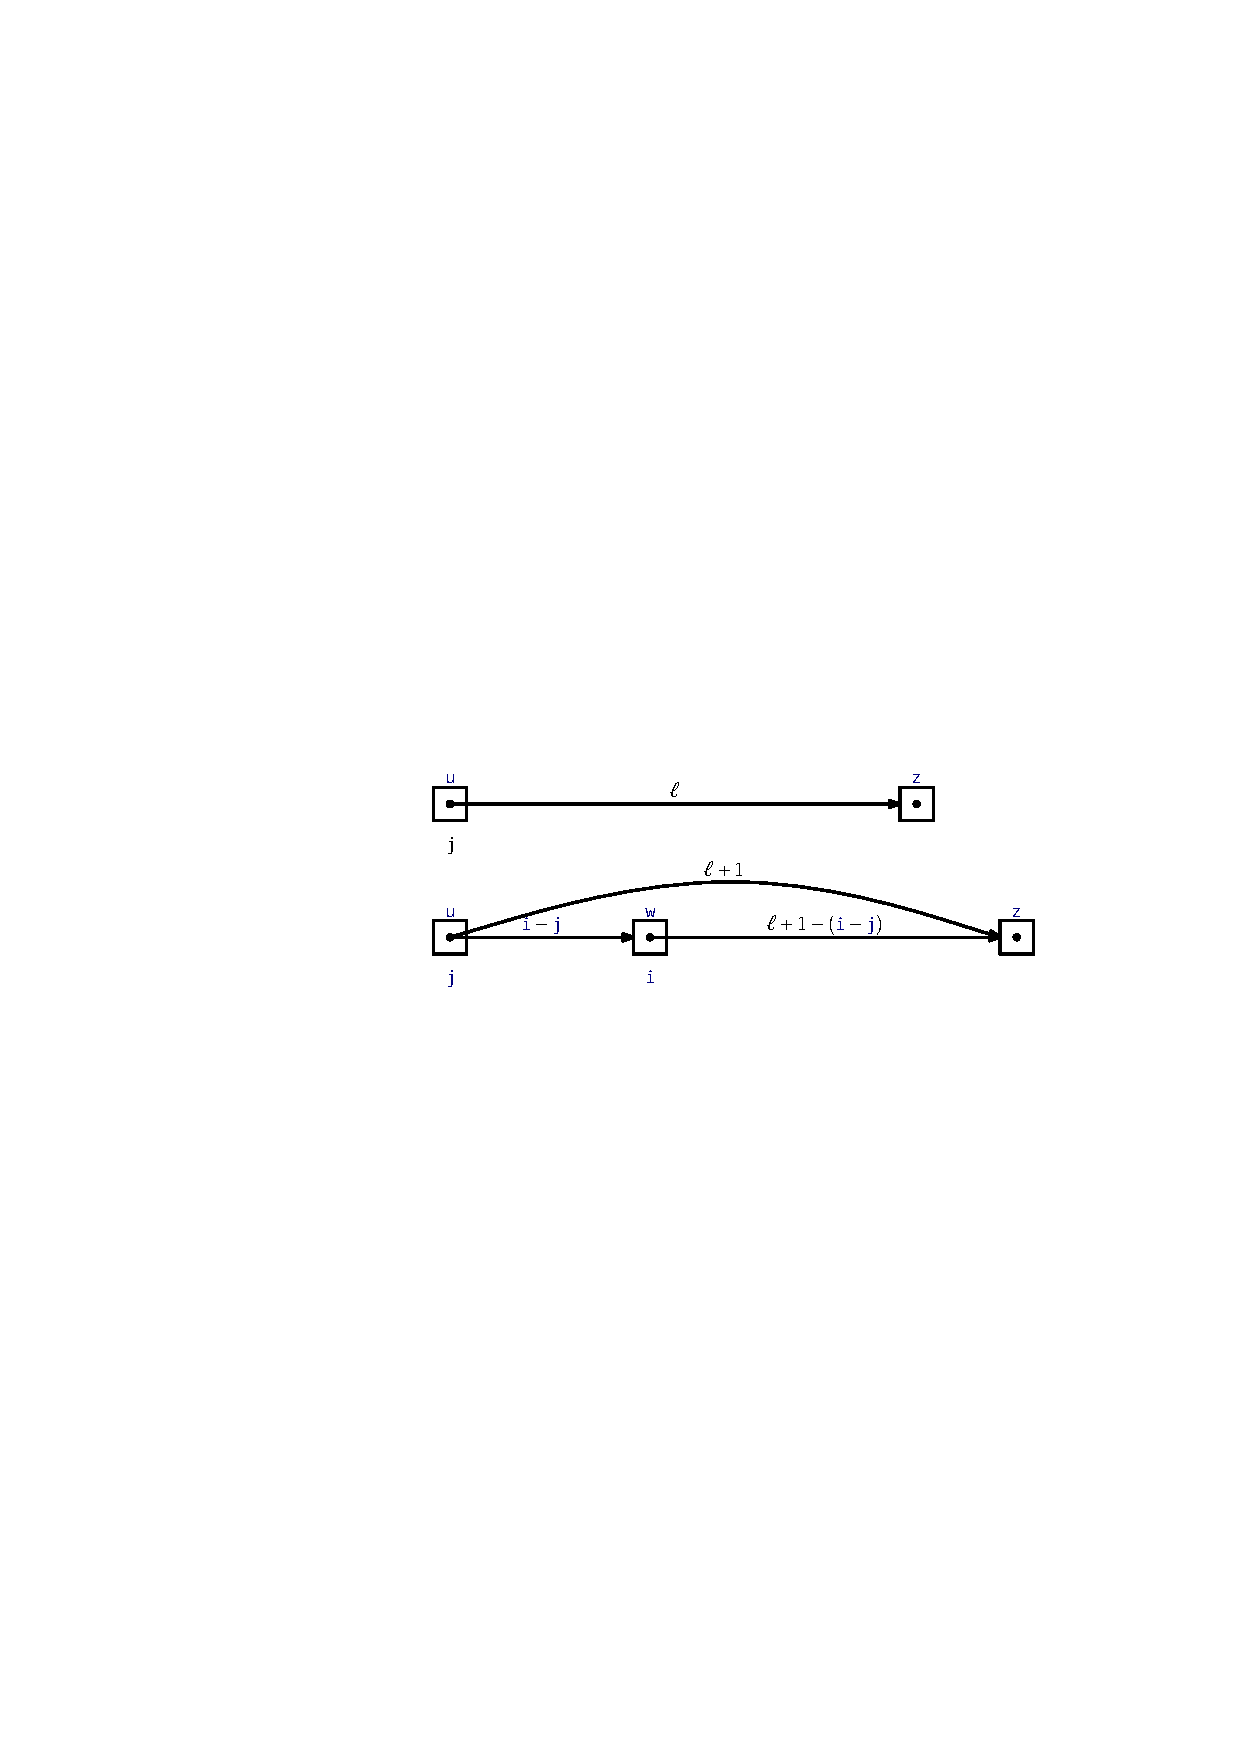
\includegraphics[scale=0.90909]{figs/skiplist-lengths-splice}
	\end{center}
	\caption[Adding to a SkiplistList]{Atualizando os comprimentos das arestas enquanto junta-se o nó 
		#w# em uma skiplist.}
	\figlabel{skiplist-lengths-splice}
\end{figure}

Isto soa mais complicado do que é, o código, na verdade, 
é bem simples:

\codeimport{ods/SkiplistList.add(i,x)}
\codeimport{ods/SkiplistList.add(i,w)}


Até agora, a implementação da 
operação #remove(i)# em uma #SkiplistList# deveria ser óbvia.  Seguimos o caminho de busca para o nó na posição #i#. Cada vez que o caminho de busca desce de um nó, #u#, no nível #r# diminuímos o comprimento da aresta deixando #u# neste nível.  Também checamos se #u.next[r]# é o elemento de classificação #i# e, caso seja, o tiramos da lista neste nível. Um exemplo é mostrado na \figref{skiplist-removei}.
\begin{figure}
	\begin{center}
		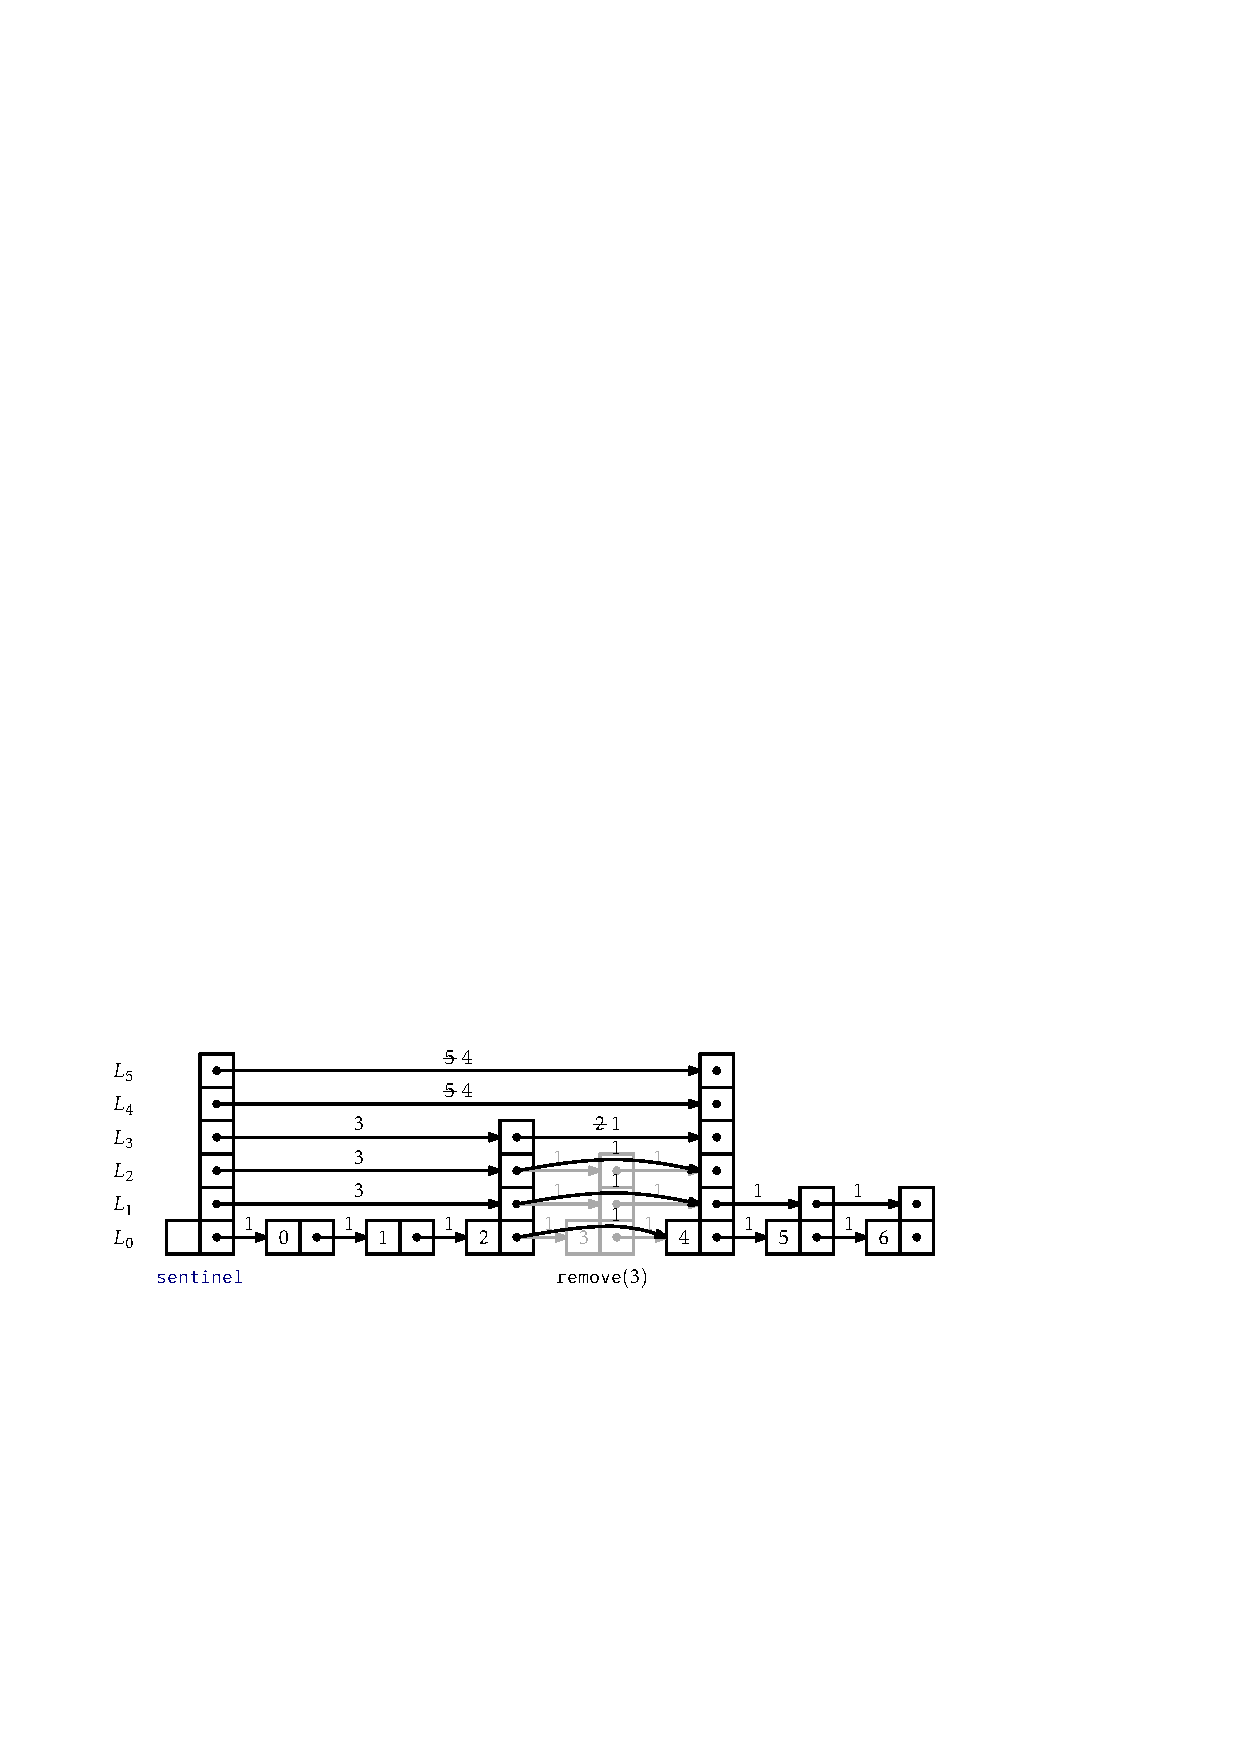
\includegraphics[width=\ScaleIfNeeded]{figs/skiplist-removei}
	\end{center}
	\caption[Removing an element from a SkiplistList]{Removing an element from a #SkiplistList#.}
	\figlabel{skiplist-removei}
\end{figure}
\codeimport{ods/SkiplistList.remove(i)}

\subsection{Resumo}

O teorema a seguir resume a performance da estrutura de dados 
#SkiplistList#:

\begin{thm}\thmlabel{skiplistlist}
	Uma #SkiplistList# implementa a interface #List#.  Uma #SkiplistList#
	suporta as operações #get(i)#, #set(i,x)#, #add(i,x)#, e
	#remove(i)# no tempo de execuçao $O(\log #n#)$ esperado.
\end{thm}

%\section{Skiplists as Ropes}
%TODO: A section on ropes

\section{Análise de Skiplists}
\seclabel{skiplist-analysis}

Nesta seção, analizamos a altura, tamanho e comprimento esperados do
caminho de busca em uma skiplist. Esta seção requer um conhecimento de
probabilidade básica.  Várias provas são baseadas nas seguintes observações
básicas sobre lançamentos de moedas.

%inicio Leonardo
\begin{lem}\lemlabel{coin-tosses}
  \index{lançamentos de moeda}%
  Faça com que $T$ seja o número de vezes que uma moeda é jogada e incluindo
  a primeira vez que a moeda dá cara.  Logo $\E[T]=2$.
\end{lem}

\begin{proof}
   Suponhamos que paremos de jogar a moeda na primeira vez que a moeda der
	 cara. Define-se a variável indicadora
	 \[ I_{i} = \left\{\begin{array}{ll}
	 0 & \mbox{se a moeda for lançada menos que $i$ vezes} \\
	 1 & \mbox{se a moeda for lançada $i$ ou mais vezes} 
	 \end{array}\right.
	 \]
	 Note que $I_i=1$ se e apenas se, o primeiro $i-1$ lançamento da moeda der coroa,
	 então $\E[I_i]=\Pr\{I_i=1\}=1/2^{i-1}$.  Observe que $T$, o número total de lançamentos da moeda, pode ser escrito como $T=\sum_{i=1}^{\infty} I_i$.
	 Portanto,
  \begin{align*}
    \E[T] & =  \E\left[\sum_{i=1}^\infty I_i\right] \\
     & =  \sum_{i=1}^\infty \E\left[I_i\right] \\
     & =  \sum_{i=1}^\infty 1/2^{i-1} \\
     & =  1 + 1/2 + 1/4 + 1/8 + \cdots \\
     & =  2 \enspace .   \qedhere
  \end{align*} 
\end{proof}

Os dois próximos lemas nos dizem que as skiplists têm tamanho linear:

\begin{lem}\lemlabel{skiplist-size1}
	O número esperado de nós em uma skiplist contendo $#n#$ elementos,
	não incluindo ocorrências do sentinela, é $2#n#$.
\end{lem}

\begin{proof}
	A probabilidade de que qualquer elemento particular, #x#, esteja incluso na lista
	$L_{#r#}$ é $1/2^{#r#}$, então o número de nós esperado na $L_{#r#}$
	é $#n#/2^{#r#}$.\footnote{Veja \secref{randomization} para ver como isso é derivado usando variáveis indicadoras e linearidade de expectativa.}
	Portanto, o número total de nós esperado em todas as listas é
	\[ \sum_{#r#=0}^\infty #n#/2^{#r#} = #n#(1+1/2+1/4+1/8+\cdots) = 2#n# \enspace . \qedhere \]
\end{proof}

\begin{lem}\lemlabel{skiplist-height}
	A altura esperada de uma skiplist contendo #n# elements é no máximo
	$\log #n# + 2$.
\end{lem}

\begin{proof}
	Para cada $#r#\in\{1,2,3,\ldots,\infty\}$, 
	defina a variável indicadora aleatória  
	\[ I_{#r#} = \left\{\begin{array}{ll}
	0 & \mbox{se $L_{#r#}$ é vazia} \\
	1 & \mbox{se $L_{#r#}$ não é vazia}
	\end{array}\right.
	\]
	A altura, #h#, da skiplist é dada por
	\[
	#h# = \sum_{r=1}^\infty I_{#r#} \enspace .
	\]
	Note que $I_{#r#}$ nunca é maior que o tamanho, $|L_{#r#}|$, de $L_{#r#}$, assim 
	\[
	\E[I_{#r#}] \le \E[|L_{#r#}|] = #n#/2^{#r#} \enspace .
	\]
	Portanto, teremos
  \begin{align*}
       \E[#h#] &= \E\left[\sum_{r=1}^\infty I_{#r#}\right] \\
        &= \sum_{#r#=1}^{\infty} E[I_{#r#}] \\
        &= \sum_{#r#=1}^{\lfloor\log #n#\rfloor} E[I_{#r#}]
                 + \sum_{r=\lfloor\log #n#\rfloor+1}^{\infty} E[I_{#r#}]  \\
        &\le \sum_{#r#=1}^{\lfloor\log #n#\rfloor} 1
                 + \sum_{r=\lfloor\log #n#\rfloor+1}^{\infty} #n#/2^{#r#} \\
        &\le \log #n#
                 + \sum_{#r#=0}^\infty 1/2^{#r#} \\
        &= \log #n# + 2 \enspace . \qedhere
  \end{align*}
\end{proof}

\begin{lem}\lemlabel{skiplist-size2}
	O número esperado de nós em uma skiplist contendo $#n#$ elementos,
	incluindo todas as ocorrências do sentinela, é $2#n#+O(\log #n#)$.
\end{lem}
%fim Leonardo

%inicio Antonio Felipe
\begin{proof}
  By \lemref{skiplist-size1}, the expected number of nodes, not
  including the sentinel, is $2#n#$.  The number of occurrences of
  the sentinel is equal to the height, $#h#$, of the skiplist so, by
  \lemref{skiplist-height} the expected number of occurrences of the
  sentinel is at most $\log #n#+2 = O(\log #n#)$.
\end{proof}



\begin{lem}
The expected length of a search path in a skiplist is at most $2\log #n# + O(1)$.
\end{lem}

\begin{proof}
  The easiest way to see this is to consider the \emph{reverse search
  path} for a node, #x#.  This path starts at the predecessor of #x#
  in $L_0$.  At any point in time, if the path can go up a level, then
  it does.  If it cannot go up a level then it goes left.  Thinking about
  this for a few moments will convince us that the reverse search path for
  #x# is identical to the search path for #x#, except that it is reversed.

  The number of nodes that the reverse search path visits at a particular
  level, #r#, is related to the following experiment:  Toss a coin.
  If the coin comes up as heads, then move up and stop. Otherwise, move
  left and repeat the experiment.  The number of coin tosses before
  the heads represents the number of steps to the left that a reverse
  search path takes at a particular level.\footnote{Note that this
  might overcount the number of steps to the left, since the experiment
  should end either at the first heads or when the search path reaches
  the sentinel, whichever comes first. This is not a problem since the
  lemma is only stating an upper bound.} \lemref{coin-tosses} tells us
  that the expected number of coin tosses before the first heads is 1.

  Let $S_{#r#}$ denote the number of steps the forward search path takes at level
  $#r#$ that go to the right.   We have just argued that $\E[S_{#r#}]\le
  1$.  Furthermore, $S_{#r#}\le |L_{#r#}|$, since we can't take more steps
  in $L_{#r#}$ than the length of $L_{#r#}$, so
  \[
    \E[S_{#r#}] \le \E[|L_{#r#}|] = #n#/2^{#r#} \enspace .
  \]
  We can now finish as in the proof of \lemref{skiplist-height}.
  Let $S$ be  the length of the search path for some node, #u#, in a
  skiplist, and let $#h#$ be the height of the skiplist.  Then
  \begin{align*}
      \E[S] 
         &= \E\left[ #h# + \sum_{#r#=0}^\infty S_{#r#} \right] \\
         &= \E[#h#] + \sum_{#r#=0}^\infty \E[S_{#r#}]  \\
         &= \E[#h#] + \sum_{#r#=0}^{\lfloor\log #n#\rfloor} \E[S_{#r#}] 
              + \sum_{#r#=\lfloor\log #n#\rfloor+1}^\infty \E[S_{#r#}] \\
         &\le \E[#h#] + \sum_{#r#=0}^{\lfloor\log #n#\rfloor} 1
              + \sum_{r=\lfloor\log #n#\rfloor+1}^\infty #n#/2^{#r#} \\
         &\le \E[#h#] + \sum_{#r#=0}^{\lfloor\log #n#\rfloor} 1
              + \sum_{#r#=0}^{\infty} 1/2^{#r#} \\
         &\le \E[#h#] + \sum_{#r#=0}^{\lfloor\log #n#\rfloor} 1
              + \sum_{#r#=0}^{\infty} 1/2^{#r#} \\
         &\le \E[#h#] + \log #n# + 3 \\
         &\le 2\log #n# + 5  \enspace . \qedhere
  \end{align*}
\end{proof}


The following theorem summarizes the results in this section:
\begin{thm}
A skiplist containing $#n#$ elements has expected size $O(#n#)$ and the
expected length of the search path for any particular element is at most
$2\log #n# + O(1)$.
\end{thm}



%\section{Iteration and Finger Search}

%TODO: Write this section

\section{Discussion and Exercises}

Skiplists were introduced by Pugh \cite{p91} who also presented
a number of applications and extensions of skiplists \cite{p89}.  Since then they
have been studied extensively.  Several researchers have done very
precise analyses of the expected length and variance of the length of the
search path for the #i#th element in a skiplist \cite{kp94,kmp95,pmp92}.
Deterministic versions \cite{mps92}, biased versions \cite{bbg02,esss01},
and self-adjusting versions \cite{bdl08} of skiplists have all been
developed.  Skiplist implementations have been written for various
languages and frameworks and have been used in open-source database
systems \cite{skipdb,redis}. A variant of skiplists is used in the HP-UX
operating system kernel's process management structures \cite{hpux}.
\javaonly{Skiplists are even part of the Java 1.6 API \cite{oracle_jdk6}.}
%fim Antonio Felipe

\begin{exc}
	Explique os caminhos de pesquisa para 2.5 e 5.5 na skiplist da \figref{skiplist}.
\end{exc}

\begin{exc}
	Explique a adição dos valores 0,5 (com uma altura de 1) e 3,5 (com uma altura de 2) na skiplist da \figref{skiplist}.
\end{exc}

\begin{exc}
	Explique a remoção dos valores 1 e 3 na skiplist da \figref{skiplist}.
\end{exc}

\begin{exc}
	Explique a execução de #remove(2)# na #SkiplistList# da \figref{skiplist-lengths}.
\end{exc}

\begin{exc}
	Ilustre a execução de #add(3,x)# na #SkiplistList# da \figref{skiplist-lengths}, assumindo que o método #pickHeight()# seleciona uma altura de 4 para o nó recém-criado.
\end{exc}

\begin{exc}\exclabel{skiplist-changes}
	Mostre que, durante uma operação #add(x)# ou #remove(x)#, o número esperado de ponteiros em #SkiplistSet# que são alterados é constante.
\end{exc}

\begin{exc}\exclabel{skiplist-opt}
	Suponha que, em vez de promover um elemento de $L_{i-1}$ para $L_i$ com base num lançamento de moeda, promovamos com alguma probabilidade $p$, $0 < p < 1$.
	\begin{enumerate}
		\item Mostre que, com esta modificação, o comprimento esperado de um caminho de pesquisa é no máximo $(1/p)\log_{1/p} #n# + O(1)$.
		\item Qual é o valor de $p$ que minimiza a expressão anterior?
		\item Qual é a altura esperada da skiplist?
		\item Qual é o número esperado de nós na skiplist?
	\end{enumerate}
\end{exc}


\begin{exc}\exclabel{skiplist-opt-2}
	O método #find(x)# em uma #SkiplistSet# às vezes executa \emph{comparações redundantes}; estas ocorrem quando #x# é comparado com o mesmo valor mais de uma vez. Elas podem ocorrer quando, para algum nó, #u#, $#u.next[r]# = #u.next[r-1]#$. Mostre como essas comparações redundantes acontecem e modifique #find(x)# para que elas sejam evitadas. Analise o número esperado de comparações feitas pelo seu método #find(x)# modificado.
\end{exc}

\begin{exc}
	Projete e implemente uma versão de uma skiplist que implemente a interface #SSet#, mas também permite acesso rápido a elementos por classificação. Ou seja, ele também suporta a função #get(i)#, que retorna o elemento cuja classificação é #i# no tempo esperado $O(\log #n#)$. (A classificação de um elemento #x# em um #SSet# é o número de elementos no #SSet# que são menores que #x#.)
\end{exc}

\begin{exc}
	\index{finger}%
	\index{finger search!in a skiplist}%
	Um \emph{indicador} em uma skiplist é um array que armazena a sequência de nós em um caminho de busca no qual o caminho de busca evolui. (A variável #pilha# no código de #add(x)# na página ~\pageref{pg:skiplist-add} é um indicador, os nós sombreados na \figref{skiplist-add} mostram o conteúdo do indicador). Pode-se pensar em um dedo apontando o caminho para um nó na lista mais baixa, $L_0$.
	
	Uma \emph{busca por indicador} implementa a operação #find(x)# usando um indicador que percorre a lista até alcançar um nó #u#, tal que $#u.x# < #x#$ e $#u.next#=#null#$ ou $#u.next.x# > #x#$, e em seguida realiza uma pesquisa normal para #x# a partir de #u#.
	É possível provar que o número esperado de passos necessários para uma pesquisa por indicador é $O(1+\log r)$, onde $r$ é o número de valores em $L_0$ entre #x# e o valor apontado pelo indicador.
	
	Implementar uma subclasse de #Skiplist# chamada #SkiplistWithFinger# que implementa operações #find(x)# usando um indicador interno. Esta subclasse armazena um indicador, que é então usado para que cada operação #find(x)# seja implementada como uma pesquisa de indicador. Durante cada operação #find(x)#, o indicador é atualizado para que cada operação #find(x)# use, como ponto de partida, um indicador que aponte para o resultado da operação #find(x)# anterior.
\end{exc}

\begin{exc}\exclabel{skiplist-truncate}
	Escreva um método, #truncate(i)#, que trunca uma #SkiplistList# na posição #i#. Após a execução deste método, o tamanho da lista é #i# e contém apenas os elementos nos índices $0,\ldots,#i#-1$. O valor de retorno é outra #SkiplistList# que contém os elementos nos índices $#i#,\ldots,#n#-1$. Esse método deve ser executado em um tempo $O(\log#n#)$.
\end{exc}

\begin{exc}
	Escreva um método #SkiplistList#, #absorb(l2)#, que toma como argumento uma #SkiplistList#, #l2#, esvazia-a e anexa seu conteúdo, em ordem, ao receptor. Por exemplo, se #l1# contiver $a, b, c$ e #l2# contém $d, e, f$, depois de chamar #l1.absorb(l2)#, #l1# conterá $a, b, c, d, e, f$ e #l2# estará vazia. Esse método deve ser executado em um tempo $O(\log#n#)$.
\end{exc}

\begin{exc}
	Usando as idéias da lista eficiente em termos de espaço, #SEList#, projete e implemente um #SSet# eficiente em espaço, #SESSet#. Para fazer isso, armazene os dados, em ordem, em uma #SEList#, e armazene os blocos desta #SEList# em um #SSet#. Se a implementação #SSet# original usa $O(#n#)$ espaço para armazenar #n# elementos, então #SESSet# usará espaço suficiente para #n# elementos mais $O(#n#/#b#+#b#)$ espaço perdido.
\end{exc}

\begin{exc}
	Usando #SSet# como sua estrutura subjacente, projete e implemente um aplicativo que leia um arquivo de texto (grande) e permita pesquisar, de forma interativa, qualquer subcadeia contida no texto. À medida que o usuário digita sua consulta, uma parte correspondente do texto (se houver) deve aparecer como resultado.
	
	\noindent Dica 1: Cada substring é um prefixo de algum sufixo, então basta armazenar todos os sufixos do arquivo texto.
	
	\noindent Dica 2: Qualquer sufixo pode ser representado de forma compacta como um inteiro simples indicando onde o sufixo começa no texto.
	
	\noindent Teste sua aplicação em alguns textos grandes, como alguns dos livros disponíveis no Project Gutenberg \cite{gutenberg}. Se for feito corretamente, suas aplicações serão bem responsivas; não deve haver atraso notável entre as teclas de digitação e os resultados.
\end{exc}

\begin{exc}
  \index{skiplist!versus binary search tree}%
  \index{binary search tree!versus skiplist}%
  (Este exercício deve ser feito depois de ler sobre árvores de busca binária, em \secref{binarysearchtree}.) Compare as skiplists com árvores de pesquisa binária das seguintes maneiras:
  \begin {enumerate}
  \item Explicar como a remoção de algumas arestas de uma skiplists leva a uma estrutura que se parece a uma árvore binária e é semelhante a uma árvore de pesquisa binária.
  \item Skiplists e árvores de pesquisa binária usam cada uma o mesmo número de ponteiros (2 por nó). As skiplists fazem um melhor uso desses ponteiros. Explique o porquê.
  \end{enumerate}
\end{exc}